\normaltrue \difficilefalse \tdifficilefalse
\correctiontrue

%\UPSTIidClasse{11} % 11 sup, 12 spé
%\newcommand{\UPSTIidClasse}{11}

\exer{Moteur à courant continu$\star$ \label{B2:04:51}}
\setcounter{numques}{0}
\UPSTIcompetence[2]{B2-04}
\index{Compétence B2-04}
\index{Fonctions de transfert}
\index{Moteur à courant continu}
\index{MCC}
\ifcorrection
\else
\textbf{Pas de corrigé pour cet exercice.}
\fi


\ifprof 
\else
On donne les équations du moteur à courant continu :
\begin{itemize}
\item $u(t) = e(t)+ Ri(t) +L \dfrac{\text{d}i(t)}{\text{d} t}$;
\item $e(t)=K\omega(t)$;
\item $c(t)=Ki(t)$;
\item $c(t)- f\omega(t)=J\dfrac{\text{d}\omega(t)}{\text{d} t}$.
\end{itemize}
\fi

\question{Exprimer la fonction de transfert $H(p)=\dfrac{\Omega(p)}{U(p)}$.}
\ifprof
En passant les équations dans le domaine de Laplace, on a : 
\begin{itemize}
\item $U(p) = E(p)+ RI(p) +LpI(p)$;
\item $E(p)=K_m\Omega(p)$;
\item $C(p)=K_mI(p)$;
\item $C(p)- f\Omega(p)=Jp\Omega(p)$ $\Leftrightarrow C(p)=\Omega(p)\left( Jp +f \right)$.
\end{itemize}

\textbf{Vous devez savoir qu'un moteur à courant continu est piloté en tension ($U(p)$) et qu'en sortie on observe le taux de rotation ($\Omega(p)$). }

En ne conservant que $U(p)$ et $\Omega(p)$, on a donc
$U(p) = E(p)+ RI(p) +LpI(p)$
$ \Leftrightarrow U(p) = K_m\Omega(p)+ \left(R +Lp\right)\dfrac{C(p)}{K_m}$
$ \Leftrightarrow U(p) = K_m\Omega(p)+ \left(R +Lp\right)\dfrac{\Omega(p)\left( Jp +f \right)}{K_m}$
$ \Leftrightarrow U(p) = \left(K_m+ \left(R +Lp\right)\dfrac{\left( Jp +f \right)}{K_m}\right)\Omega(p)$
$ \Leftrightarrow U(p) =  \dfrac{K_m^2 + \left(R +Lp\right)\left( Jp +f \right)}{K_m}\Omega(p)$.

On a donc $H(p)=\dfrac{\Omega(p)}{U(p)}$ $=\dfrac{K}{K^2 +\left(R +Lp\right) \left( Jp +f \right)} $.

%\begin{figure}[H]
%\centering
%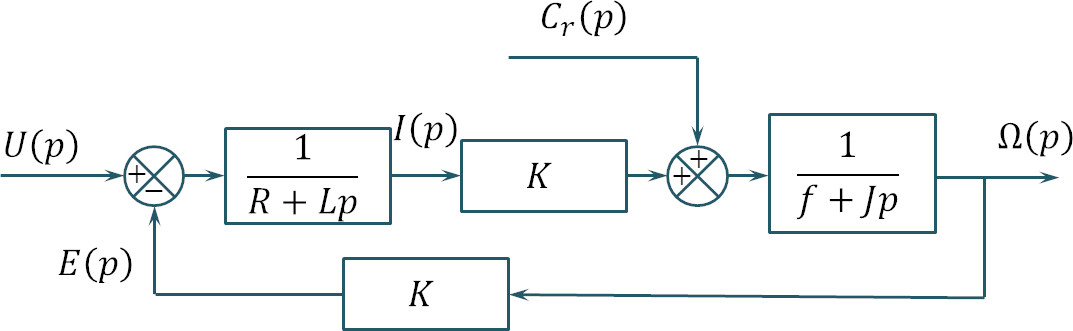
\includegraphics[width=\linewidth]{51_01_c}
%\caption{Évolution du couple utile en fonction de la vitesse de rotation pour des
%fréquences de commande de \SI{90}{Hz} à \SI{110}{Hz}. \label{fig_50_04}}
%\end{figure}
\else
\fi

\question{Préciser l'ordre et la classe de $H$.}
\ifprof
$H$ est d'ordre 2 et de classe 0 car on ne peut pas mettre de $p$ en facteur. Le terme de plus haut degré du dénominateur est de degré 2. 
\else
\fi

\question{Mettre $H(p)$ sous forme canonique.}
\ifprof
$H(p)=\dfrac{K_m}{K_m^2+ Rf +\left(RJ  + Lf\right) p + LJp^2 } $
$\Leftrightarrow H(p)=\dfrac{\dfrac{K_m}{K_m^2+ Rf}}{1 +\dfrac{\left(RJ  + Lf\right)}{K_m^2+ Rf} p + \dfrac{LJ}{K_m^2+ Rf}p^2 } $. 

\else
\fi




\question{Donner les caractéristiques de la fonction de transfert.}
\ifprof
En identifiant avec la forme canonique standard, $H(p)=\ordredeux$ soit
$K = \dfrac{K_m}{K_m^2+ Rf}$, $\dfrac{2\xi}{\omega_0} = \dfrac{\left(RJ  + Lf\right)}{K_m^2+ Rf}$ et $\dfrac{1}{\omega_0^2}=\dfrac{LJ}{K_m^2+ Rf}$.


Au final,
$K = \dfrac{K_m}{K_m^2+ Rf}$,
$\omega_0=\sqrt{\dfrac{K_m^2+ Rf}{LJ}}$,
$\xi = \dfrac{RJ  + Lf}{2\sqrt{{LJ\left(K_m^2+ Rf\right)}}}$.
\else
\fi

\question{Vérifier l'homgénéité des différentes constantes.}
\ifprof

Le gain doit être en $\si{rad.s^{-1}V^{-1}}$.

D'une part, $[K_m]=\si{N.m.A^{-1}}$. D'autre part, $[K_m]=\si{V.rad^{-1}.s}$. On a donc $\si{V.rad^{-1}.s}=\si{N.m.A^{-1}}$. (On pourrait aussi le montrer par une analyse dimensionnelle...)

De plus $[R]=\Omega = \dfrac{\si{V}}{\si{A}}$ et $[f]=\si{N.m.rad^{-1}.s}$.

On a donc 
$[K]=\dfrac{\si{N.m.A^{-1}}}
{(\si{N.m.A^{-1}})^2+\si{N.m.rad^{-1}.s}\times\si{VA^{-1}} }$
$=\dfrac{1}
{\si{N.m.A^{-1}}+\si{rad^{-1}.s.V} }$
$=\dfrac{1} {\si{rad^{-1}.s.V} }$
$= {\si{rad.s^{-1}.V^{-1}} }$. 

\vspace{.5cm}

La pulsation propre doit être en $\si{s^{-1}}$ ou $\si{rad.s^{-1}}$.

On a vu que $[K_m^2] = [Rf]$. De plus $[L] = H =  \si{V.s.A^{-1}}$ et 
$[J]=\si{Nm.rad^{-1}s^2}$ (PFD).

$[\omega_0]=\sqrt{
\dfrac{\si{N^2.m^2.A^{-2}}}
{\si{V.s.A^{-1}} \times \si{Nm.rad^{-1}s^2}}
}$
$=\sqrt{
\dfrac{\si{N.m.rad}}{\si{V.s.A.s^2}}
}$. 
Or, $\si{W}=\si{N.m.rad.s^{-1}}=\si{VA}$.

On a alors 
$[\omega_0]=\sqrt{
\dfrac{\si{N.m.rad.s^{-1}}}{\si{V.s^2.A}}
}$
$=\sqrt{
\dfrac{1}{\si{s^2}}
}=\si{s^{-1}}$.


Enfin, $\xi$ est sans unité... à vérifier :)
%
%
%
%$[\xi]=  \dfrac{\si{N.m.rad^{-1}.s}\si{Nm.rad^{-1}s^2}  + \si{V.s.A^{-1}}\si{N.m.rad^{-1}.s}}{\sqrt{{\si{V.s.A^{-1}}\si{Nm.rad^{-1}s^2} \si{N.m.rad^{-1}.s}\si{N.m.rad^{-1}.s}}}}$
%$=  \dfrac{\si{N.m.rad^{-1}.s}\si{Nm.rad^{-1}s^2}  + \si{V.s.A^{-1}}\si{N.m.rad^{-1}.s}}{\si{N.m.rad^{-1}.s}\sqrt{{\si{V.s.A^{-1}}\si{Nm.rad^{-1}s^2} }}}$
%$=  \dfrac{\si{Nm.rad^{-1}s^2}  + \si{V.s.A^{-1}}}
%{\sqrt{{\si{V.s.A^{-1}}\si{Nm.rad^{-1}s^2} }}}$.
%
%Or, $\si{W}=\si{N.m.rad.s^{-1}}=\si{VA}$; donc $\si{N.m}=\si{VA.rad^{-1}.s}$; donc 
%
%
%$[\xi]=  \dfrac{\si{VA.rad^{-1}.s.rad^{-1}s^2}  + \si{V.s.A^{-1}}}
%{\sqrt{{\si{V.s.A^{-1}}\si{VA.rad^{-1}.s.rad^{-1}s^2} }}}$
%$=  \dfrac{\si{VA.rad^{-2}s^3}  + \si{V.s.A^{-1}}}
%{\sqrt{{\si{V^2.rad^{-2}s^4} }}}$
%$=  \dfrac{\si{VA.rad^{-2}s^3}  + \si{V.s.A^{-1}}}
%{\si{V.rad^{-1}s^2} }$
%$=  \dfrac{\si{A.rad^{-2}s^2}  + \si{V.A^{-1}}}
%{\si{rad^{-1}s} }$
%$=  \dfrac{\si{A^2.rad^{-2}s^2}  + \si{V}}
%{\si{A.rad^{-1}s} }$

\else
\fi




\ifprof
\else

\ifcolle
\else
\noindent\footnotesize
\fbox{\parbox{.9\linewidth}{
Éléments de corrigé : 
\begin{enumerate}
    \item $H(p)=\dfrac{K_m}{K_m^2 +\left(R +Lp\right) \left( Jp +f \right)} $.
    \item Ordre 2, classe 0.
    \item $H(p)=\dfrac{\dfrac{K_m}{K_m^2+ Rf}}{1 +\dfrac{\left(RJ  + Lf\right)}{K_m^2+ Rf} p + \dfrac{LJ}{K_m^2+ Rf}p^2 } $.
    \item $K = \dfrac{K_m}{K_m^2+ Rf}$,
$\omega_0=\sqrt{\dfrac{K_m^2+ Rf}{LJ}}$,
$\xi = \dfrac{RJ  + Lf}{2\sqrt{{LJ\left(K_m^2+ Rf\right)}}}$.
\end{enumerate}}}
\normalsize
\fi

\begin{flushright}
\footnotesize{Corrigé  voir \ref{B2:04:51}.}
\end{flushright}%
\fi